%aum gaanathipathaye namaha
%srj
\section{Pre-Processing Phase}\label{sec:pre-proc}

\todo {\color{blue} write 1-2 lines about what is going to happen here}

%\subsection{Preprocessing}
\subsection{Disassembly of Binaries}
%\hfill \break \hfill
We first obtain the disassembly of signature and target programs. Then, each program is split into functions and finally, from each function, we construct the control-flow graphs (CFG), where each CFG is consists of one or more basic-blocks. The definitions of CFG and basic-block are given below:

\mydef{(Basic-block) A sequence of assembly instructions without any jumps or jump targets in the middle, where jump targets start a block, and jumps end a block.}
\mydef{(Control-flow graph) A directed graph, where each node represents a basic-block and edges represent control flow transitions.}

\subsection{Synthetic Feature Extraction} \label{subsec:syn_fea}
%These code properties act as contextual information for the vulnerability. 

%\todo {\color{blue} Define code property and explain each of the following in details with some examples.}
In general, the real world application are fairly large, where the number of functions can easily exceed several thousands. For example, openssl (version 1.0.1f) for Windows, compiled using Mingw32, contains 5877 functions. However, it is expensive to perform vulnerability matching over the entire functions in the target program. Thus, it is vital to have some sort of pre-filtering process that selects only a handful of \textit{candidate functions}, from the target program, for vulnerability matching. Here, candidate function refers to the function that is likely to have the vulnerability that we are searching for. In our system, we use the synthetic features (or \textit{code properties}) of the vulnerability signature to filter the target functions.

In our system, we extract several code properties from the vulnerability signature based on which the target functions are ranked and the suitable candidate functions are selected for vulnerability matching. We are considering three types of code properties; (1) library call invocations, (2) operation type, and (3) structural information, and they are explained below:

\begin{itemize} 
\item \textbf{Library call invocation}: library call invocations gives valuable hints about the activities that are likely to be carried out in a function. For example, presences of \texttt{strcpy} function from \texttt{glibc} library indicates that the function is likely to handle strings. Thus, if a particular library call is present in a vulnerability signature, we can safely prune the target functions that fail to invoke the given library function.    

\item \textbf{Operation type}: Here, we look into the actual assembly code to infer the possible operations that a functions can perform. To this end, we have identified several types of operations based on the instruction mnemonics.They are as follows: data movement (e.g., \texttt{movs}), arithmetic operation (e.g., \texttt{mul}), logic operation (e.g., \texttt{and}), shift and rotate operation (e.g., \texttt{shld}), string operation (e.g., \texttt{scasb}), control-transfer operation (e.g., \texttt{jo}), explicit access to eflags (e.g., \texttt{cld}) and halt operation (e.g., \texttt{hlt}).
   
\item \textbf{Structural information}: This include cyclomatic complexity of the function, where it reflects the complexity of a function through measuring the number of linearly independent paths present, presence of loop/nested loop and other function invocations. These information roughly summaries the structural properties of a vulnerability function.

\end{itemize}

\todo {\color{blue}mention about specially crafting the features and ignoring the common ones.}
Thought these code properties helps to identify potential candidate functions in the target program, there are several drawbacks that we need to be aware of. First, it is important to note that some programs may implement their own version of some the library functions, in which case, we may fail to detect the vulnerabilities in functions (if present) that invoke their own version of library function. Fortunately, most of programs still use the standard library functions and thus, we decided to include them as part of the pre-filtering properties. Next, structural information, cannot always be trusted as, in practise, compilers can inline/outline functions and hence, this metric will provide some misleading information. Similarly, operation type may too provide some false indication as some tasks can be achieved with semantically equivalent instruction that belongs two different types in our categorization.

However, considering the number of functions present in the real world applications, it is very beneficial, in terms of scalability, to have a pre-filtering process in place to select candidate target functions that are likely to contain vulnerability.   Hence, to reduce the negative impact of our properties, we apply weights to each property based on their contribution in pre-filtering. Through evaluation, we identified that library call invocation and operation type properties considerably contributes towards correctly identifying candidate target functions followed by structural property. Therefore, the total synthetic similarity ($sim_{tot}$) is measured as follows: 
\begin{equation} 
sim_{tot} = w_l*sim_l + w_o*sim_o + w_s*sim_s \label{eq:tot_syn_sim}
\end{equation}
where, $sim_l$, $sim_o$ and $sim_s$ refers to similarities based library call invocation, operation type and structural properties, and $w_l$, $w_o$ and $w_s$ refers to their corresponding weights, respectively.

\subsection{Vulnerability Modelling} \label{subsec:vul_mod}
\begin{figure}[t]
	\centering
	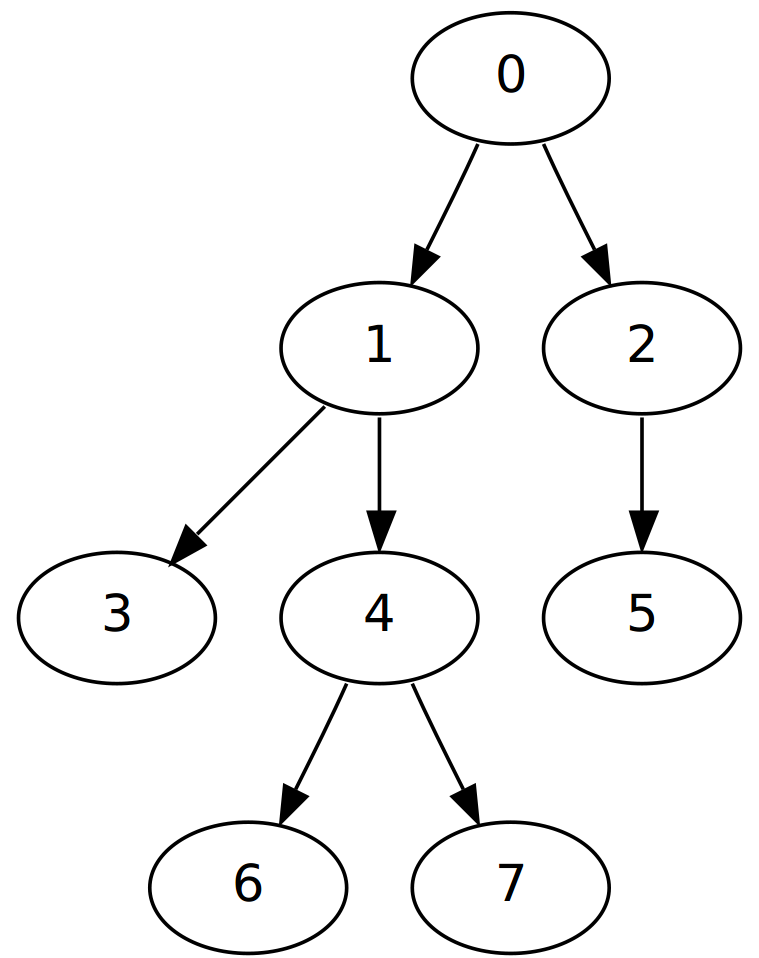
\includegraphics[width=.15\textwidth]{srj-figures/tracelet.png}
	\caption{Control-flow graph (CFG) example}\label{fig:tracelet}
\end{figure}
In contrast to basic-block centric vulnerability models proposed in the literature \cite{lakhotia2013fast}\cite{pewny2014leveraging}\cite{pewnycross}, in our system, we use a \textit{tracelet} model. Tracelet is \textit{continuous}, \textit{short}, \textit{partial} traces of an execution \cite{david2014tracelet}.
%is a sequence of adjacent basic-blocks that lie along a program execution path. 
It is observed that basic-blocks that are part of a vulnerability, in a function, likely to lie close to each other along the execution path. However, there are some odd cases that doesn't adhere to this assumption. 
%For example, \todo{provide use-after-free example}, 
However, in general, this is a reasonable assumption \cite{pewnycross}\cite{pewny2014leveraging}. Hence, tracelet models suits well to represent most of the vulnerabilities. Sample tracelet models, for $k=1,2,3$, extracted from a CFG (shown in figure \ref{fig:tracelet}) is presented in table \ref{tab:tracelet}

%talk about basic-block terminators? 

\begin{table}[t]
\caption{Tracelet models extracted from sample CFG shown in figure \ref{fig:tracelet}}\label{tab:tracelet}
\begin{center}
{\scriptsize
\begin{tabular}{|c|c|}
  \hline 
  $k$ & $k$-tracelet models \\ 
  \hline 
  1 & $\langle 0 \rangle$, $\langle 1 \rangle$, $\langle 2 \rangle$, $\langle 3 \rangle$, $\langle4\rangle$, $\langle 5 \rangle$, $\langle 6 \rangle$, $\langle 7 \rangle$\\ 
  \hline 
  2 & $\langle 0,1 \rangle$, $\langle 1,3 \rangle$, $\langle 1,4 \rangle$, $\langle 4,6 \rangle$, $\langle 4,7 \rangle$, $\langle 0,2 \rangle$, $\langle 2,5 \rangle$\\ 
  \hline 
  3 & $\langle 0,1,3 \rangle$, $\langle 1,4,6 \rangle$, $\langle 1,4,7 \rangle$, $\langle 0,2,5 \rangle$\\ 
  \hline 
  \end{tabular}    
}
\end{center}
\end{table}

\mydef{(tracelet \cite{david2014tracelet}) A tracelet is a partial execution trace that represents a single partial flow through the program. In a $k$-tracelet, $k$ denotes the number of basic-blocks in the tracelet}   

One of the advantages of tracelet model is that it is resilient to basic-block splitting and merging  that can negatively influence the vulnerability matching. Unfortunately, compiler optimizations and difference in build environments often lead to changes in the basic-block structure. Thus, basic-block based vulnerability modelling is not preferred\footnote{when we say basic-block based modelling, we refer to basic-block centric vulnerability models}.  For example, given a vulnerability signature that consists of a single basic block, if we compare each basic-block in the target function with the signature, we still may miss the vulnerability (assuming that the target function is also vulnerable) as the vulnerable code segment in the target function might have split into two (or more) basic-blocks (A real-world example is shown in figure \ref{fig:prob_stat}). That is, when the vulnerable code segment in the target function is split into several small basic-blocks, the similarity between them and the signature drops considerably, which leads to a wrong conclusion that vulnerability is not present in the target function. Similarly, basic-block merging may also lead to wrong conclusion.

However, this situation is less likely to affect our vulnerability models as the functions are modelled using $k$-tracelets, where $k$ can take the values $1$ to $n$ ($n\in\mathbb Z_{> 0}$). For example, in the above scenario, when $k=2$ (i.e., \textit{2}-tracelet model), the two adjacent basic-blocks in the target functions are merged into a single basic-block, which nullifies the effect of basic-block splitting. Similarly, given a vulnerability signature consists of three basic-blocks and in the vulnerable target function, they are merged into a single basic-block,  we still can detect the vulnerability by using \textit{3}-tracelet models to represent the vulnerability signature, which again nullifies the effects of basic-block merging. 
%That is for each tracelet in the vulnerability signature, we start searching, in the target function, from $1$-tracelet models upto $n$-tracelet models.

In the original tracelet model, proposed in \cite{david2014tracelet}, tracelet length is bounded to some value $k$ determined by the analyst. However, in our case, it is harder to manually determine the length of the tracelts (i.e., $k$) for each vulnerability. Thus, to bring flexibility and reduce the manual efforts in our modelling, the length of tracelets is not fixed for both signature ($k^s$) and target ($k^t$) programs . That is, we allow the signature and target programs to systematically adopt a suitable length for tracelets that can better represent a given vulnerability. The self-adaptable nature allows the signature and target programs to choose two different tracelet models (i.e., $k^s \neq k^t$) for the same vulnerability, which alleviates the problem caused by structural difference, at basic-block level, in the analysed programs. Later, in section \ref{sec:nns}, we'll explain how the tracelet lengths are selected for a given vulnerability in detail (please refer to Algorithm \ref{alg:nns}).  
 
\subsection{Semantic Feature Extraction} \label{subsec:sem_fea}

Here, we capture the effects of tracelets on the state of the program. A program-state, in general, can be characterised by \texttt{Register}, \texttt{Control flag} and \texttt{Memory} values. Formally, it is defined by a triple of the form:
$\langle RegMap, FlagMap, MemMap \rangle$
, where $RegMap$, $FlagMap$, and $MemMap$ map each register, control flag, and memory location in the state, respectively, to a value. Effects of each tracelet, on the program-state, is represented by a set of symbolic formulae, called \textit{symbolic expressions}.

\mydef{(Symbolic Expression) Symbolic formulae that represent the effects of a piece of code, on the program-state, in-terms of system registers, control flags and memory values.}
\begin{eqnarray}
\label{eq:sym_exp}
 \text{\texttt{push ebp}} &\equiv& \text{\texttt{ESP' = ESP-4}} ~\wedge \nonumber \\
   &&  \text{\texttt{[ESP-4] = EBP}}~
\end{eqnarray}
For example, the symbolic expression of an instruction `\texttt{push ebp}' is shown in equation \ref{eq:sym_exp} (assuming its a IA-32 machine), where we can see that when \texttt{EBP} register is pushed into the stack, the value of \texttt{ESP} register changes to \texttt{ESP-4} and the memory location \texttt{[ESP-4]} is now holding the value of \texttt{EBP} register. Here, prime (\texttt{'}) indicates the program-state post execution.  

In contrast to other symbolic expression\footnote{symbolic expression and semantic features are used interchangeably in this paper.} based program representation techniques (\cite{pewnycross}, \cite{lakhotia2013fast} and \cite{ruttenberg2014identifying}), we extract semantic features at various granularity levels to measure the effect of tracelet models at different program points. That is, in $k$-tracelet modelling, when $k=1$, semantic features (i.e., symbolic expressions) are extracted from each basic-block. Similarly, for $k=2$, the two basic-blocks, in the \textit{2}-tracelet, are combined into one code block, from which, the symbolic expressions are extracted. Essentially, depending on the length of the tracelets, the granularity of symbolic expressions are varied. 

Figure \ref{fig:sym_expr_granu} depicts the sample basic-blocks (assuming they are adjacent) and the corresponding symbolic expressions extracted for \textit{1}- and \textit{2}-tracelet models. From the example, it can be seen that \texttt{ESP}, \texttt{EBX} and \texttt{ECX} registers hold different values in \textit{2}-tracelet model (see figure ?) compare to \textit{1}-tracelet model (see figure ? and ?). That is, when two basic-blocks are merged, the extracted semantic features change considerably, which in return, will have an adversarial effect in vulnerability signature matching process. Thus, it is vital to extract semantic features at a suitable granularity level such that the vulnerabilities are not missed. 

\begin{figure}
\centering
\noindent
\begin{minipage}{.11\textwidth}
\begin{lstlisting}[caption=BB1,frame=tlrb]{Name}
push ebp
mov ebp, esp
\end{lstlisting}
\end{minipage}\hfill
\begin{minipage}{.11\textwidth}
\begin{lstlisting}[caption=BB2,frame=tlrb]{Name}
pop ebx
mov ecx, ebx 
\end{lstlisting}
\end{minipage}\hfill
\begin{minipage}{.15\textwidth}
\begin{lstlisting}[caption=sym. expr for BB1 (1-tracelet model),frame=tlrb]{Name}
ESP' = ESP - 0x4
[ESP - 0x4] = EBP
EBP = ESP - 0x4
\end{lstlisting}
\end{minipage}\hfill

\begin{minipage}{.15\textwidth}
\begin{lstlisting}[caption=sym. expr for BB2 (1-tracelet model),frame=tlrb]{Name}
ESP' = ESP + 0x4
EBX = [ESP]
ECX = [ESP]
\end{lstlisting}
\end{minipage}\hfill
\begin{minipage}{.20\textwidth}
\begin{lstlisting}[caption=sym. expr for both BBs combined (2-tracelet model),frame=tlrb]{Name}
ESP' = ESP - 0x4 + 0x4 
[ESP - 0x4] = EBP
EBP = ESP - 0x4
EBX = [ESP - 0x4]
ECX = [ESP - 0x4]
\end{lstlisting}
\end{minipage}
\caption{Sample basic-blocks and their corresponding symbolic expressions at two different granularity levels \todo {\color{blue} need to fix this figure alignment}. }\label{fig:sym_expr_granu}
\end{figure}


%\todo {\color{blue} provide example for symbolic expression}.

%\subsection{Vulnerability Signature Matching}

